\documentclass[11pt]{article}
\usepackage{mathtools}
\usepackage{mdframed}
\usepackage{fullpage}
\usepackage{amsfonts}
\usepackage{tikz}
\usepackage{fancyhdr}
\usepackage{lastpage}
\usetikzlibrary{automata, positioning}


%edit this for each class
\newcommand\name{John Collin Vincent}
\newcommand\classname{Com S 331}
\newcommand\assignment{Homework 8}


\newcounter{excounter}
\setcounter{excounter}{1}
\newcommand\ques[2]{\vskip 1em  \noindent\textbf{\arabic{excounter}\addtocounter{excounter}{1}.} \emph{#1} \noindent#2}
\newenvironment{question}{\ques{}\begin{quote}}{\end{quote}}


\pagestyle{fancy}
\rfoot{\name, page \thepage/\pageref{LastPage}}
\cfoot{}
\rhead{}
\lhead{}
\renewcommand{\headrulewidth}{0pt}
\renewcommand{\footrulewidth}{0pt}
\DeclarePairedDelimiter\ceil{\lceil}{\rceil}
\DeclarePairedDelimiter\floor{\lfloor}{\rfloor}


\begin{document}


  {\bf \classname \hspace{1cm} \assignment\hfill \name}
  \vskip 2em


  \begin{question}
    \center
    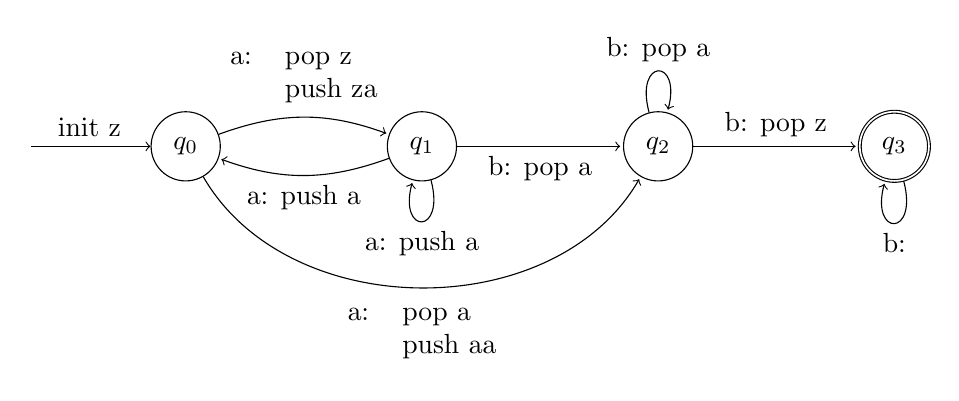
\begin{tikzpicture}[shorten >=1pt,node distance=3cm,on grid,auto]
      \node[state] (q_0) {$q_0$};
      \node[state] (q_1) [right=of q_0] {$q_1$};
      \node[state] (q_2) [right=of q_1] {$q_2$};
      \node[state, accepting] (q_3) [right=of q_2] {$q_3$};
      \draw[<-] (q_0) -- node[above] {init z} ++(-2cm, 0);
      \path[->]
      (q_0) edge [bend left=20] node [above] {\begin{tabular}{ll}a:&pop z\\&push za\end{tabular}} (q_1)
            edge [bend right=60] node [below] {\begin{tabular}{ll}a:&pop a\\&push aa\end{tabular}} (q_2);
      \path[->]
      (q_1) edge [loop below] node [below] {a: push a} ()
            edge [bend left=20] node [below] {a: push a} (q_0)
            edge node [below] {b: pop a} (q_2);
      \path[->]
      (q_2) edge [loop above] node [above] {b: pop a} ()
            edge  node [above] {b: pop z} (q_3);
      \path[->]
      (q_3) edge [loop below] node [below] {b: } ();
    \end{tikzpicture}
  \end{question}

  \begin{question}
    consider the string $w=b^ma^{m+1}b^m$ when applying the pumping lemma to this string there are really three distinct
    ways of decomposing $w$ into $uv^kxy^kz, vy\ne\epsilon, |vxy|\le m$. One way is where both $v$ and $y$ are comprised of a run of b's,
    which would look like, $b^{m-i-j}b^{ik}b^{jk}a^{m+1}b^m$ or $b^ma^{m+1}b^{m-i-j}b^{ik}b^{jk}$ or $b^{m-i}b^{ik}a^{m+1}b^{m-j}b^{jk}$ where $i,j\geq1, i\le j$,
    all of these fail to pump because when $k=2$ one of the run's of b is at least $m+i$ and $m+i\geq m+1$. The second way to split $w$ would
    be to have $u=b^i, y=a^j$ which would result in $b^{m-i}b^{ik}a^{m+1-j}a^{jk}b^{m}$ and when $k=0, |a|_w = m+1-j$ and one set of b's is of length $m$ still and
    $m+1-j\le m$; this version is symetric to if $y=a^j, u=b^i$ and $u$ was in the second run of b's. The third option is that $u=a^i, y^j$ which would result
    in $b^ma^{m+1-j-i}a^{jk}a^{ik}b^{m}$ when $k=0$ the run of a's is at most $m+1-j-i$ which is less than both run's of b which is $m$ showing that this valid
    string $w\in L$ does not pump so $L$ is not context free.
  \end{question}

  \begin{question}
    by contradiciton if $L$ was a CFL then there must be a way to partition $\forall w\in L$ so that $uvxyz, |v||y|\geq 1, |vxy|\le m$ pumps.
    Consider $w= 1^m0^m21^{m+1}0^{m-1}$, we know that $v,y$ cannot contain $2$ because then when $k=0$ the string does not contain a two and is not in the language.
    If both $u,y$ are on the left side then pumping 2 times will result in $\alpha$ having a 1 in a higher place value making
    $\lbrack\alpha\rbrack_2 > \lbrack\beta\rbrack_2$. Then same would be true if both $v$ and $y$ are on the right side of the 2 and $k=0$ since at least
    two characters will be removed from the right string making $\lbrack\alpha\rbrack_2 > \lbrack\beta\rbrack_2$. If $v$ is on the right and $y$ is on the
    left then when $|v| < |y|$ pumping $0$ times will result in $|\alpha| > |\beta|\implies\lbrack\alpha\rbrack_2 > \lbrack\beta\rbrack_2$, when
    $|v| > |y|$ pumping 2 times will result in the same, and when $|v| = |y| = i \geq 1$ pumping 0 times will result in
    $1^m0^{m-i}21^{m+1-i}0^{m-1}$ which results in $\lbrack\alpha\rbrack_2 = \lbrack\beta\rbrack_2$ when $i=1$ and
    $\lbrack\alpha\rbrack_2 > \lbrack\beta\rbrack_2$ when $i>1$. So in no partition does $w$ pump and since $w\in L, L$ is not context free.
  \end{question}

\end{document}
